\section{Our Method}
\label{sec:method}

In this section, we present \textbf{CMVKG-Guard}, a novel framework designed to detect and mitigate hallucinations in Vision-Language Models (VLMs) in real-time. Unlike prior approaches that rely on static knowledge bases or post-hoc corrections, our method dynamically constructs a Hierarchical Multimodal Knowledge Graph (DH-MMKG) during inference and employs a multi-layered verification engine.

\begin{figure*}[t]
    \centering
    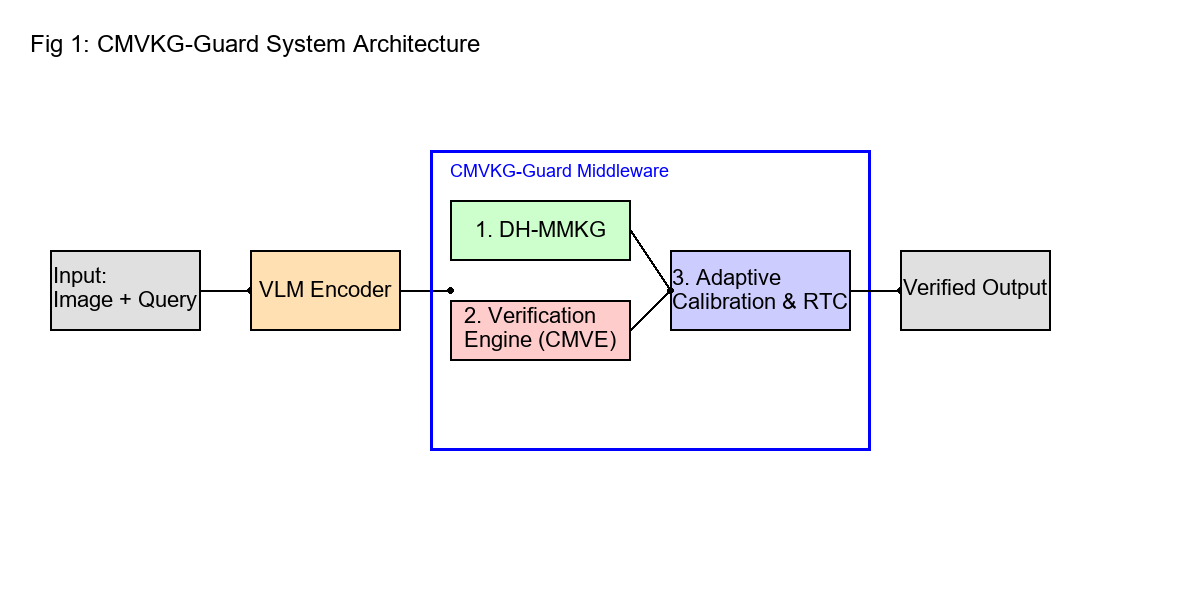
\includegraphics[width=\linewidth]{figures/system_architecture.png}
    \caption{Overview of the CMVKG-Guard architecture. The framework acts as a middleware, intercepting VLM output and verifying it against a dynamically constructed Hierarchical Multimodal Knowledge Graph (DH-MMKG) using a Cross-Modal Verification Engine (CMVE).}
    \label{fig:system_arch}
\end{figure*}

\subsection{Problem Formulation}
Let $\mathcal{M}$ be a Vision-Language Model parameterized by $\theta$. Given an image $I$ and a textual query $Q$, the model generates a response sequence $R = \{t_1, t_2, ..., t_T\}$, where $t_i \in \mathcal{V}_{vocab}$ represents the $i$-th token. The autoregressive generation probability is defined as:
\begin{equation}
P(R | I, Q) = \prod_{i=1}^{T} P(t_i | I, Q, t_{<i}; \theta)
\end{equation}
where $t_{<i}$ denotes the sequence of tokens generated prior to step $i$.

We define the \textit{hallucination detection} task as learning a binary decision function $f_{\text{ver}}: \mathcal{V}_{vocab} \times \mathcal{I} \times \mathcal{K} \to \{0, 1\}$, where $1$ indicates a hallucination. The function relies on a dynamic knowledge source $\mathcal{K}$ constructed on-the-fly. If $f_{\text{ver}}(t_i) = 1$, a correction function $f_{\text{corr}}$ maps $t_i$ to a grounded token $t^*_i$.

\subsection{Dynamic Hierarchical Multimodal Knowledge Graph (DH-MMKG)}
To address the limitations of static knowledge bases, we introduce the DH-MMKG, formally denoted as $\mathcal{G} = (\mathcal{V}, \mathcal{E}, \mathcal{S})$, where $\mathcal{V}$ is the set of entity nodes, $\mathcal{E}$ is the set of relational edges, and $\mathcal{S}$ represents the global scene context.

\subsubsection{Visual Scene Graph Construction ($L_1$)}
The base layer $L_1$ captures visual primitives. We employ an open-vocabulary object detector $D$ to extract a set of objects $O = \{o_1, ..., o_N\}$. For each object $o_j$, we extract a feature vector $\mathbf{v}_j$ and a set of attributes $\mathcal{A}_j = \{(a_k, s_k)\}_{k=1}^{K}$, where $a_k$ is an attribute label (e.g., "red") and $s_k$ is the confidence score.

The set of edges $\mathcal{E}_{vis}$ represents spatial relationships derived from bounding box geometry. Let $B(o_i)$ be the bounding box of object $o_i$. The spatial relation $r_{sp}(o_i, o_j)$ is determined by:
\begin{equation}
r_{sp}(o_i, o_j) = \psi_{\text{geo}}(B(o_i), B(o_j))
\end{equation}
where $\psi_{\text{geo}}$ is a geometric heuristic function mapping to predicates such as $\{\text{left\_of}, \text{above}, \text{inside}\}$.

\begin{figure}[h]
    \centering
    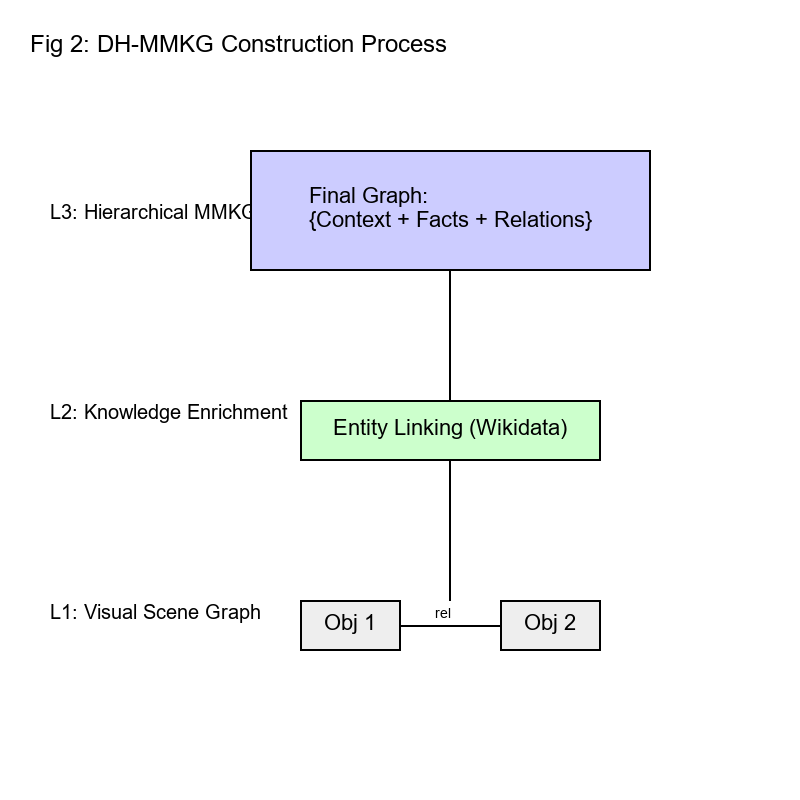
\includegraphics[width=0.9\linewidth]{figures/dh_mmkg_process.png}
    \caption{Construction process of the Dynamic Hierarchical Multimodal Knowledge Graph (DH-MMKG).}
    \label{fig:dh_mmkg_process}
\end{figure}

\subsubsection{Knowledge Enrichment ($L_2$)}
The second layer $L_2$ enriches $\mathcal{G}$ with external factual knowledge by actively querying APIs. We define a linking function $\Phi: \mathcal{V} \to \mathcal{K}_{ext}$ that maps visual entities to an aggregate external knowledge base comprising both Wikidata (fetching ontological properties via SPARQL, such as `instance of` or `subclass of`) and ConceptNet (fetching relational bindings).

For each linked entity $e_j = \Phi(o_j)$, we retrieve a subgraph $\mathcal{G}_{sub}(e_j) \subset \mathcal{K}_{ext}$ subject to a relevance constraint based on the query embedding $\mathbf{q}$:
\begin{equation}
\mathcal{G}_{sub}(e_j) = \{ (e_j, r, e') \in \mathcal{K}_{ext} \mid \text{sim}(\mathbf{e}(r), \mathbf{q}) > \delta \}
\end{equation}
This ensures that only contextually relevant facts are added to the DH-MMKG. A local disk-caching mechanism is implemented to maintain low-latency query resolution without exhausting external rate limits during large-scale evaluation benchmarking. Importantly, this knowledge enrichment layer also mitigates potential error propagation from the open-vocabulary detector in $L_1$. If a visually detected object is spurious, its inability to form coherent factual links in the external knowledge bases reduces its prominence in the resulting graph, effectively serving as early filtering of detection errors. To maintain scalability and handle inherent conflicts, visual evidence is configured to strictly override textual facts.

\begin{algorithm}
\caption{DH-MMKG Construction Algorithm}
\label{alg:dh_mmkg}
\begin{algorithmic}[1]
\Require Image $I$, Query $Q$, Threshold $\delta$
\Ensure Graph $\mathcal{G}$
\State $O \leftarrow \text{Detector}(I)$
\State $\mathcal{V} \leftarrow \emptyset, \mathcal{E} \leftarrow \emptyset$
\For{$o_j \in O$}
    \State $\mathcal{A}_j \leftarrow \text{AttributeExtractor}(o_j, I)$
    \State $\mathcal{V} \leftarrow \mathcal{V} \cup \{ \text{Node}(o_j, \mathcal{A}_j) \}$
\EndFor
\For{$o_i, o_j \in O$}
    \State $r_{sp} \leftarrow \psi_{\text{geo}}(B(o_i), B(o_j))$
    \State $\mathcal{E} \leftarrow \mathcal{E} \cup \{ (o_i, r_{sp}, o_j) \}$
\EndFor
\For{$v \in \mathcal{V}$}
    \State $e \leftarrow \Phi(v)$
    \State $\mathcal{F} \leftarrow \text{RetrieveFacts}(e, Q, \delta)$
    \State $\mathcal{G} \leftarrow \text{Merge}(\mathcal{G}, \mathcal{F})$
\EndFor
\State \Return $\mathcal{G}$
\end{algorithmic}
\end{algorithm}

The time complexity of the DH-MMKG construction is primarily bounded by the number of detected objects $N$ and the retrieval fan-out $k$. Assuming constant time for embedding comparisons, the overall time complexity is $\mathcal{O}(N^2 + N \log k)$. This bounded complexity ensures the extraction pipeline induces minimal latency overhead during real-time inference.

\noindent\textbf{KG update mechanism.} The DH-MMKG is constructed once per query before generation begins. During the token-by-token generation loop, the graph is treated as a read-only grounding source. If the model generates a new named entity that was not in the initial visual scene (e.g., an inferred off-screen object), a lightweight incremental update appends that entity node and fetches its immediate one-hop facts from the cache. This avoids re-running the full $\mathcal{O}(N^2)$ construction and adds only $\mathcal{O}(\log k)$ per newly encountered entity.

\noindent\textbf{Conflict resolution.} When the external knowledge facts $\mathcal{F}$ conflict with visually detected attributes (e.g., Wikidata says ``fire trucks are red'' but the detected object is blue), we apply a strict visual-priority rule: the edge contributed by $L_1$ detection is assigned confidence weight $w_{vis} = 1.0$ and overrides the external edge, which is downweighted to $w_{ext} = 0.2$. This prevents hallucination by external knowledge sources while still retaining them as weak soft constraints.

\noindent\textbf{Scalability.} For open-domain queries with many detected entities ($N > 20$), we cap external knowledge retrieval to the top-5 most query-relevant entities (ranked by cosine similarity between entity embedding and query embedding), ensuring the graph remains compact and query-time graph search stays bounded. Caching of API responses (Wikidata SPARQL, ConceptNet) means repeated entity lookups across a session incur zero network latency.


\subsection{Cross-Modal Verification Engine (CMVE)}
The CMVE verifies each generated token $t_i$ against $\mathcal{G}$ and $I$.

\subsubsection{Layer 1: Visual-Textual Alignment}
We compute the Visual Attention Ratio (VAR). Let $\mathbf{A}_l \in \mathbb{R}^{T \times S}$ be the cross-attention map at layer $l$, where $S$ is the number of visual tokens. The attention weight of token $t_i$ on visual patch $s_j$ is given by $\alpha_{i,j}$. The VAR score is:
\begin{equation}
\text{VAR}(t_i) = \frac{1}{L} \sum_{l=1}^{L} \sum_{j=1}^{S} \alpha_{i,j}^{(l)} \cdot \mathbb{1}(s_j \in \text{ROI}(t_i))
\end{equation}
To prevent the language prior from dominating the semantic alignment, we introduce a \textbf{Counterfactual Contrastive Validator}. We dynamically generate a semantic counterfactual $t_{cf}$ (e.g., an antonym or mutually exclusive token) and compute a delta similarity. The final visual score $S_{vis}(t_i)$ is then computed as:
\begin{equation}
S_{vis}(t_i) = \lambda_1 \text{VAR}(t_i) + \lambda_2 \max\left(0, \text{sim}(t_i, \text{img}) - \text{sim}(t_{cf}, \text{img})\right)
\end{equation}
where $\text{sim}(t, \text{img})$ denotes the standard CLIP-based cosine similarity. This ensures that a token is only granted a high visual score if it strictly discriminates itself from its counterfactual, effectively neutralizing absolute baseline probabilities caused by language biases.

\subsubsection{Layer 2: Knowledge Grounding}
For a token $t_i$ identified as a named entity, we check for its existence in $\mathcal{G}$. If $t_i \in \mathcal{V}$, we evaluate the path validity score. Let $\mathcal{P}_{t_i}$ be the set of paths from context entities to $t_i$ in $\mathcal{G}$. The score is:
\begin{equation}
S_{kg}(t_i) = \max_{p \in \mathcal{P}_{t_i}} \left( \prod_{(u,v) \in p} w(u,v) \right)
\end{equation}
where $w(u,v)$ is the confidence of the edge.

\subsubsection{Layer 3: Reasoning Chain Verification}
Beyond factual correctness, we verify logical consistency using a structural entailment approach modeling multi-hop dependencies. Given a candidate token $t_i$ representing an action or state, we evaluate its validity using the context representations in $\mathcal{G}$:
\begin{equation}
S_{logic}(t_i) = \sigma \left( \sum_{p \in \mathcal{T}_{t_i}} \phi(p) \cdot \mathbb{I}(t_i \models p) \right)
\end{equation}
\begin{equation}
S_{reason}(t_i) = \max \left( S_{logic}(t_i), \text{BFS}(t_i, \mathcal{G}, d_{max}) \right)
\end{equation}
where $\mathcal{T}_{t_i}$ is the set of logical predicates extracted from the local context, $\phi(p)$ is the heuristic path weight, and $\mathbb{I}$ is the entailment indicator function modeled via robust morphological string similarity techniques against graph edges. Additionally, a generic Breadth-First Search (BFS) graph traversal function executes up to $d_{max}=3$ hops from the candidate token to capture multi-hop cascading reasoning dependencies in structurally complex generated text.

\subsubsection{Unified Verification Score (UVS)}
The final verification score $\Omega(t_i)$ is a weighted combination of individual module scores:
\begin{equation}
\Omega(t_i) = \mathbf{w}^T \cdot [S_{vis}(t_i), S_{kg}(t_i), S_{reason}(t_i)]
\end{equation}
where $\mathbf{w} = [w_1, w_2, w_3]$ with default values $[0.30, 0.40, 0.30]$ (empirically set to reflect the relative discriminative power of each layer). Crucially, $\mathbf{w}$ is \textbf{not} learned via any gradient-based update. Instead, it is \textit{heuristically re-weighted at inference time} by classifying the incoming query into one of three types—structural (high $w_1$), factual (high $w_2$), or logical (high $w_3$)—using lightweight keyword-matching against the query string. This re-weighting is a deterministic, rule-based function with no trainable parameters, fully preserving the training-free property of the framework.

\noindent\textbf{Is CMVE differentiable?} No. The entire CMVE is a non-differentiable, heuristic verification layer. $S_{vis}$ relies on attention thresholding and CLIP cosine similarity; $S_{kg}$ uses graph path products; $S_{reason}$ uses BFS traversal and string-matching similarity. None of these operations involve learned parameters or gradient flow. CMVE is therefore structurally suitable for plug-and-play middleware integration with any frozen VLM.

\begin{figure}[t]
    \centering
    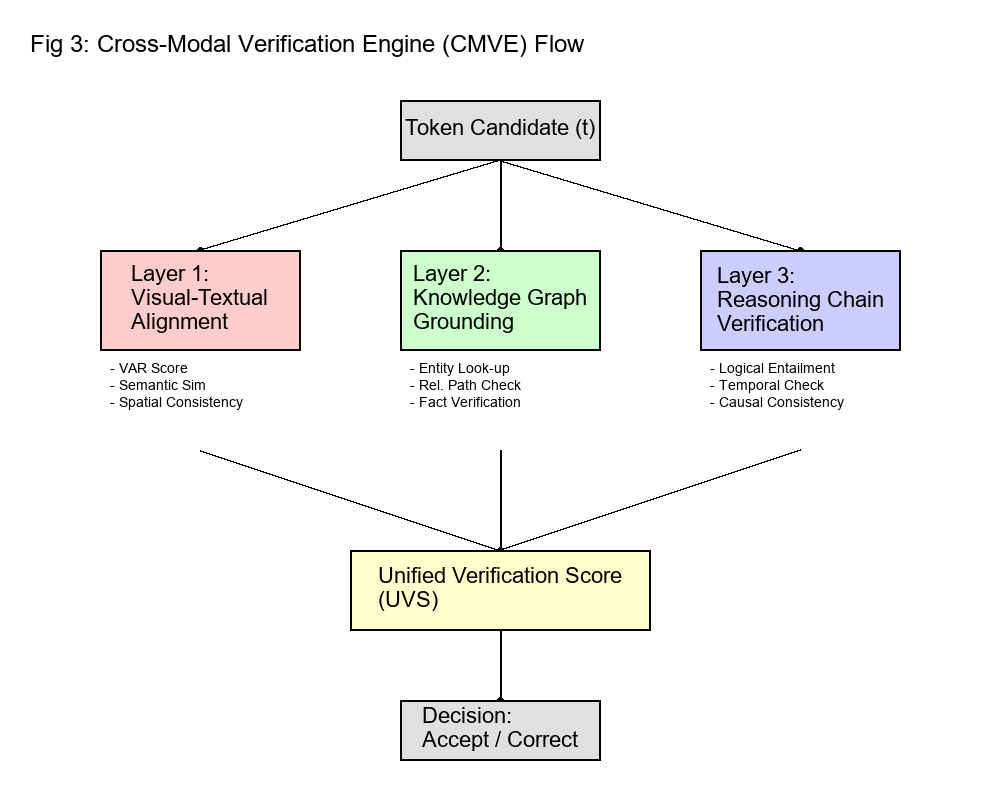
\includegraphics[width=\linewidth]{figures/cmve_verification_flow.png}
    \caption{Workflow of the Cross-Modal Verification Engine (CMVE). For each speculative token $t_i$, the three verification layers compute $S_{vis}$, $S_{kg}$, and $S_{reason}$ independently and in parallel. These are combined via the heuristic weight vector $\mathbf{w}$ into the Unified Verification Score $\Omega(t_i)$, which is compared against the adaptive threshold $\tau_{dyn}$ to trigger correction if needed.}
    \label{fig:cmve_flow}
\end{figure}

\subsection{Adaptive Confidence Calibration and Real-Time Correction}
We define a dynamic threshold $\tau_{dyn}$ based not only on static context heuristics but crucially on the real-time autoregressive progression of the answer to counter hallucination ``snowballing''. The threshold dynamically increases its penalty weight using the current generation step $s$:
\begin{equation}
\tau_{dyn}(t_i) = \theta_{base} + \omega_{risk} + \omega_{complexity} + \min(\lambda, \eta \cdot s_i)
\end{equation}
where $\theta_{base}$ is a base configured strictness, $\omega_{risk}$ acts as an upward adjustment for high-risk domains, $\omega_{complexity}$ penalizes queries requiring high-density logical verification, and the sequential step modifier ensures later tokens are scrutinized heavily.

If $\Omega(t_i) < \tau_{dyn}(t_i)$, the token is flagged as a hallucination. Replacing a single token exclusively based on local node similarities risks degrading the syntactic coherence of the autoregressive context. To bridge the perception-reasoning gap, we propose a \textbf{Constrained Look-Ahead Beam Search}. 

Instead of isolating $t_i$, we retrieve the top-$K$ semantic candidates $\mathcal{C}_{cand}$ from $\mathcal{G}$ and branch the generation into a $D$-depth look-ahead tree. The optimal correction sequence $c^*$ is selected by maximizing the joint probability over the speculative sequences:
\begin{equation}
c^* = \arg\max_{c \in \mathcal{C}_{cand}} \sum_{d=0}^{D} \left( (1-\gamma) \log P_{\text{VLM}}(t_{i+d} | t_{<i}, c_{0:d}) + \gamma \log P_{\text{KG}}(c | \mathcal{G}) \right)
\end{equation}
where $P_{\text{KG}}$ is the structural likelihood derived from the DH-MMKG.

In practical implementations, token-level interception is achieved without modifying the VLM source code. Concretely, for LLaVA-1.5, we wrap the standard \texttt{generate()} call with a custom autoregressive decoding loop (illustrated in Algorithm~\ref{alg:decoding}): at each step $i$, we (1) perform a single forward pass to obtain the logit distribution over $\mathcal{V}_{vocab}$; (2) apply argmax to identify the candidate token $\hat{t}_i$; (3) pass $\hat{t}_i$ through the CMVE; and (4) if $\Omega(\hat{t}_i) < \tau_{dyn}$, we invoke the Constrained Look-Ahead Beam Search, which evaluates $K$ graph-grounded candidates each extended $D$ steps into the future, selects $c^*$, and teacher-forces $c^*$ into the sequence by directly appending it to the KV-cache. The VLM then continues autoregressively from the corrected state. This approach requires no access to model weights, activations, or training infrastructure.

\begin{algorithm}[t]
\caption{Autoregressive Decoding with CMVKG-Guard Interception}
\label{alg:decoding}
\begin{algorithmic}[1]
\Require Image $I$, Query $Q$, Graph $\mathcal{G}$, Max tokens $T$
\Ensure Corrected response $R^*$
\State $R^* \gets []$, $\text{KV} \gets \emptyset$
\For{$i = 1, \ldots, T$}
    \State $\mathbf{l}_i \gets \text{VLM.forward}(I, Q, R^*_{<i}; \text{KV})$
    \State $\hat{t}_i \gets \arg\max(\mathbf{l}_i)$
    \If{$\hat{t}_i = $ EOS} \textbf{break} \EndIf
    \State $\Omega(\hat{t}_i), \tau_{dyn} \gets \text{CMVE}(\hat{t}_i, I, \mathcal{G}), \text{Calibrator}(i)$
    \If{$\Omega(\hat{t}_i) < \tau_{dyn}$}
        \State $c^* \gets \text{LookAheadBeamSearch}(\hat{t}_i, \mathcal{G}, K, D)$
        \State $R^* \gets R^* \cup \{ c^* \}$, append $c^*$ to KV-cache
    \Else
        \State $R^* \gets R^* \cup \{ \hat{t}_i \}$, append $\hat{t}_i$ to KV-cache
    \EndIf
\EndFor
\State \Return $R^*$
\end{algorithmic}
\end{algorithm}
